\section{Analysis of the Digital Implementation of a Chaotic Deterministic-Stochastic Attractor }

\subsection{Introduction}
In the last thirty years chaotic systems have yielded a revolution
in our vision of nature as they have two contrasting features:
(1) they are deterministic because a mathematical model determines
their dynamics, but (2) because of their sensitivity to initial
conditions, the long time predictivity is lost, and consequently
they may be included in the class of stochastic systems being
studied by means of statistical tools. Actually, if chaotic
systems could be implemented with infinite precision, they would
be deterministic in the strict sense, but infinite precision is an ideal not
attainable in digital electronics.

This \emph{deterministic-stochastic duality} makes chaotic systems
specially interesting for engineering applications, as far as the
generated signals can be used as controlled noises in a wide range
of applications. However, chaotic sequences actually present
internal nonlinear correlations, making them unsuitable for being used as
``good" PRNGs. It is necessary to use randomization techniques to
improve the randomness of the series \cite{DeMicco2008}.

In digital applications the time and the state variable's
have discrete values. Time discretization enforces the use of
an algorithm to approximate the continuous time differential equations
that model the system. The simplest algorithm is the first order Euler's
method in which differentials are directly replaced by finite
increments. More elaborated algorithms, like fourth order (or
higher) constant step Runge-Kutta and variable
step algorithms, make the discrete system to evolve closer to the
continuous system, but with higher resources requirements. Consequently they must be used only if exactitude is a requirement of the specific application. This is not the case in PRNG, where randomness is the main characteristic to be guaranteed.

In order to make the arithmetical calculations, computers must internally represent
the signals by a finite number of bits, it means the values are
described using finite precision arithmetics. This restriction may
be critical for a chaotic system as it is extremely sensitive to
the arithmetic employed and can even lose its chaotic behavior.

In this paper, we implement a discrete Lorenz oscillator obtained
by using Euler's first order algorithm and three different
representation standards. We further apply  randomization
techniques to the state variables to obtain a realtime PRNG. The
aim of this work is to study the influence of the discretization
procedure on the system's dynamic. In \cite{DeMicco2010}  a
deterministic chaotic system stochasticity degree was studied by
its single-precision (32-bit) floating point ieee 754
implementation. In \cite{Wolff1986} the dynamics of contracting
integer maps is studied.

Stochasticity degree determination aims to provide a design
methodology optimized for the intended utility given to the
chaotic system. Thus, for example there are applications requiring
that the chaotic system replaces a stochastic system (cryptography
\cite{Fernandez2003}, sequence generators to spread spectrum
communications \cite{Setti2004,DeMicco2007B}, pseudorandom number
generators \cite{Kocarev2003,Larrondo2006,DeMicco2009}, reduction
of electromagnetic interference \cite{Callegari2003A}, etc.). On
the other hand, some applications require long term
predictability, i. e. to reproduce the chaotic system as accurate
as possible, this is the case for example with analog
communications using synchronization chaotic carriers
\cite{Kocarev1995,Hidalgo2001}.

Another issue is the exact determination of the pseudorandom sequence's period.
For generators that are based on
lineal operations the problem has been studied
in depth, and well known design criteria are at disposal to obtain
maximum cycle devices.   Examples of  linear algorithms are Mersenne Twister algorithm that is a
very fast random number generator  of period $2^{19937}-1$
\cite{Matsumoto1998} and Multiply-With-Carry (MWC), a method
invented by George Marsaglia for the generation of sequences of
random integers based on an initial set from two to many thousands
of randomly chosen seed values, it presents immense periods,
ranging from around $2^{60}$ to $2^{2000000}$
\cite{Marsaglia1991}. However, from the cryptographic point of
view they are weak.  When dealing with cryptographic applications,
linear methods for generating pseudo-random sequences (like LFSRs,
LCGs or their proper combinations) are highly not recommended,
since efficient algorithms are at disposal to predict the sequence
on the basis of a relatively short sequence observation
\cite{Boyar1989,Plumstead1982}. On the other hand, for most families of
nonlinear generators the problem seems to be intractable and, with few
exceptions, in the case of the non-linear systems usually
does not  exist an analitical evaluation of their periods.
\cite{kocarev2011}.

We choose the Lorenz chaotic system because it is a widely studied
system and it has also been implemented by other authors  with
different methodologies \cite{Asseri2002,Azzaz2009,Azzaz2010}.
For example in \cite{Asseri2002}, a Lorenz chaotic oscillator was
implemented by means of a toolbox of the Xilinx System Generator
that works under $MATLAB-Simulink^\copyright$. This toolbox
converts the MATLAB-Simulink model into the Xilinx System
Generator model. Then the VHDL code is obtained.
%One drawback of
%this strategy is the automatic code generation tools of VHDL are
%non-optimal,
As it is an automatic operation it does not allow
certain specific changes and presents some limitations.
The integration operation was approximated with the Euler's algorithm,
using sum and delay blocks. The implementation proposed in
\cite{Azzaz2009} and \cite{Azzaz2010} uses $RK4$ in a $32-$bit
fixed point architecture. The application considered was the
generation of chaotic random key for data stream encryption.

In this paper $Quartus$ II $7.2^\copyright$ development software
is used to generate the VHDL hardware description language    and
the physical implementation is made on the development board
$Altera^\copyright$ Cyclone III $EP3C120$. Three representations
are studied: 1)  floating-point IEEE $754$ standard, 2) decimal
fixed point, and 3) integer arithmetics  \cite{Gonzalez2003}. Each
representation involves a different number of bits.  We consider
two floating point representations for the standards single or
double, with $32$ and
 $64$ bits respectively to represent the sign, the exponent and the
mantissa; decimal fixed point arithmetics uses $p$ bits
to represent the integer part and $m$ bits to represent the
fractional part. We considered $32$ and $64$ bits fixed point representations with $9$ bits for the integer part and $1$ bit for the sign and the remaining $22$ or $54$ bits for the fractional part. In the $k$ bits integer arithmetics
the alphabet has $2^k$ symbols. We considered $k=54$.

In order to quantify the system randomness
Marsaglia's DIEHARD tests-suite is used. These tests have been widely employed in
the open literature and are very effective for classifying
deterministic and stochastic systems.

This paper is organized as follows: in section
\ref{sec:lorenzdigit} the time discretization of the continuous time chaotic system is
presented. Section \ref{sec:numrepre} describes the Lorenz
oscillator in different numeric representations: subsection \ref{sec:impleFloat} for the IEEE $754$ standard floating point representations, subsection \ref{sec:impleFix} for the fixed-point
representations
 and subsection \ref{sec:impleInt} for the integer
arithmetic implementation. Section \ref{sec:PRNG} remarks some
issues concerning the use of a chaotic systme as a PRNG and
finally in Sections \ref{sec:resultados} and \ref{sec:conclusions}
results and conclusions are presented.

%-----------------------------------------------------------------------------------------------------------
\subsection{Time discretization of the Lorenz oscillator}
\label{sec:lorenzdigit}

The Lorenz system is defined by the following set of coupled
ordinary differential equations:

%
\begin{eqnarray} \label{eq:lorconti}
\frac{dx}{dt}&=&-\delta(x-y) \ , \nonumber \\
\frac{dy}{dt}&=&\Gamma x-y-xz \ , \\
\frac{dz}{dt}&=&-bz+xy \ , \nonumber
\end{eqnarray}
%
where $\delta$, $\Gamma$ and $b$ are constructive parameters of
the system. For certain values of these constructive parameters the
system has a chaotic behavior.
%
An algorithm is always required to convert a continuous dynamical
system into a discrete time dynamical system. The simplest
algorithm was proposed by Euler and, for Eqs. \ref{eq:lorconti}
the following discrete model arises:

\begin{eqnarray}\label{eq:loreuler}
{\widetilde X}_{t+\Delta t}&=&{\widetilde X}_{t}+ \Delta t \left[
- \delta \left( {\widetilde X}_{t}-{\widetilde Y}_{t} \right)
\right]
\ , \nonumber \\
{\widetilde Y}_{t+\Delta t}&=&{\widetilde Y}_{t}+ \Delta t \left[
-{\widetilde X}_{t}{\widetilde Z}_{t}+\Gamma~{\widetilde
X}_{t}-{\widetilde Y}_{t} \right] \ ,
\\
{\widetilde Z}_{t+\Delta t}&=&{\widetilde Z}_{t}+ \Delta t \left[
{\widetilde X}_{t}{\widetilde Y}_{t}-b~{\widetilde Z}_{t} \right]
\ , \nonumber
\end{eqnarray}
%
where $\Delta t$ is the time step size and $\widetilde X$,
$\widetilde Y$, and $\widetilde Z$ are discrete time state
variables (reals).

The Euler algorithm is a one step algorithm because in order to
calculate the variables at the time $t+ \Delta t$ it is only
necessary to know the values at the previous instant. Calculating iteratively with an appropriate step $\Delta t$ it is
possible to obtain the evolution of the discrete system. It is reasonably to expect that the smaller the value of $\Delta
t$ the more exact would be the values obtained. Although, reducing
the value of $\Delta t$ leads to increment the number of
calculations and this generates more round-off errors.

In applications requiring an exact reproduction of the dynamics of
the continuous system more involved algorithms are mandatory but
in the case of PRNGs only the statistical properties and
randomness of the time series are important and consequently the
Euler algorithm is good enough.

%===================================================
\subsection{Discretization of the state variables}
\label{sec:numrepre}
As pointed out in the introduction three different numerical
representations are used in this paper. Each one is described in
the following subsections.
%----------------------------
\subsubsection{IEEE $754$ standard implementation}
\label{sec:impleFloat} Floating point representation is one of the
methods to represent real numbers with finite precision. The
advantage of floating-point representation over fixed-point and
integer representations is it can support a much wider range of
values because it automatically scales each number to use the full
word length for the mantissa; this is done by moving the decimal
point (this procedure implies a change in the value of the
exponent) towards the position of the most significant bit.
Consequently full precision is preserved even for small numbers.
Binary floating-point arithmetic is best suited to work
 with real-world quantities over a wide range of
scales. Special care must be taken because of some accuracy issues. %
%
The single precision IEEE $754$ standard assigns $23$ bits to the
mantissa (bit $0$ to $22$), the exponent occupies the following
$8$ bits (bit $23$ to $30$) and the $31$-st bit is assigned to the
sign. The double precision IEEE $754$ standard assigns $52$ bits to the
mantissa (bit $0$ to $51$), the exponent occupies the following
$11$ bits (bit $52$ to $62$) and the $63$-rd bit is assigned to the
sign.

Floating point arithmetic operations are more complicated than
fixed point ones. Their execution requires more time and complex
hardware. However, thanks to technological advance and the
development of new materials, nowadays there exists FPGAs with
more memory and resources, capable of working at high frequencies in these standards.

%--------------------------------
\subsubsection{Fixed point implementation}
\label{sec:impleFix} When all the numbers are within a known range
it is possible to achieve more accuracy using the so-called fixed
point representation instead of the floating point representation.
The hardware required to manipulate these representations is the
same commonly used to perform integer operations and it is less
expensive than the one required for the floating-point case.

To avoid the overflow it is necessary to initially perform an
analysis to determine the largest value involved in the calculus,
including the intermediate operations. With this information the
minimum number of bits to be employed is determined. Once
established the number of bits required to represent the integer
part, one additional bit is used to represent negative numbers
(based two complement). The remaining bits added are used to
improve the precision as they represent the decimal part.

The addition, substraction and multiplication operations are
implemented in the same way as in integer arithmetic. It is only
necessary to take care of the position of the radix point.

In this paper we considered two cases, $32$ and $64$ bits for each
whole number. In both cases we used $9$ bits for the integer part,
plus $1$ bit for the sign, leaving the remaining bits, $22$ or $54$ respectively,
for the decimal part.
%--------------------------------------------------------
\subsubsection{Integer arithmetics implementation}
\label{sec:impleInt}

In integer arithmetics the circuitry can be significantly reduced
if power of $2$ divisors are adopted. To obtain the integer version for the Lorenz system
the following transformations of polarization and scaling, were done
\cite{Gonzalez2003}:

\begin{eqnarray} \label{eq:newvariables}
{X}_{t}&=&\left({\widetilde X}_{t} + B\right)S \ , \nonumber \\
{Y}_{t}&=&\left({\widetilde Y}_{t} + B\right)S \ , \\
{Z}_{t}&=&\left({\widetilde Z}_{t} + B\right)S \ , \nonumber
\end{eqnarray}
%
where $B$ y $S$ are the polarization and scale parameters
respectively. Replacing eq. (\ref{eq:newvariables}) in
(\ref{eq:loreuler}) it is obtained:
%

\begin{eqnarray}\label{eq:Lorenz2}
{X}_{t+\Delta t}&=& {X}_{t} + \Delta t \ \delta~\left( {Y}_{t} -
{X}_{t} \right)
\ ,\nonumber \\
{Y}_{t+\Delta t}&=&(1- \Delta t )~{Y}_{t}+ \Delta t \
(B+\Gamma)~{X}_{t}~+~
\Delta t ~B~{Z}_{t} \nonumber\\
&~&-{\frac{\Delta t}{S}}{X}_{t}{Z}_{t}+ \Delta t \ BS(1-\Gamma-B) \ ,\\
{Z}_{t+\Delta t}&=&(1-\Delta t b){Z}_{t}-\Delta t B\left( {X}_{t}
+
{Y}_{t} \right)\nonumber \\
&&+{\frac{\Delta t}{S}}{X}_{t}{Y}_{t}+ \Delta t \ BS(B-b) \ .
\nonumber
\end{eqnarray}
%
In this paper it was adopted: \\

$\delta=8$, $\Gamma=24$, $b=2$, $\Delta t \ =2^{-n}$,
$B=40$, $S=512$. \\

Some care must be taken when the system parameters are chosen, in
this case integer coefficients were selected
% for the system implementation. A
and an analysis of stability was done in order to
ensure that the system do not converge to a fixed point or to a low
period orbit.
%
The final system is:
\begin{eqnarray}\label{eq:Lorenz3}
{X}_{t+\Delta t}&=&{X}_{t}+floor\left[ {\frac{{Y}_{t}}{2^{{n-3}}}}
\right] -floor\left[{\frac{{X}_{t}}{2^{{n-3}}}}\right] \ , \nonumber \\
{Y}_{t+\Delta t}&=&{Y}_{t}-floor\left[
{\frac{{Y}_{t}}{2^n}}\right]
+floor\left[{\frac{{X}_{t}}{2^{{n-6}}}}\right]\nonumber \\
&& +floor\left[ {\frac{{Z}_{t}}{2^{{n-3}}}}\right] +
floor\left[{\frac{{Z}_{t}}{2^{{n-5}}}}\right]\nonumber \\
&&-floor\left[ {\frac{{X}_{t}}{2^{( 22+floor\left[
{\frac{n}{2}+1}\right] )}
}}\right] \nonumber \\
&& floor\left[ {\frac{{Z}_{t}}{2^{( 22+floor\left[
{\frac{n}{2}}\right] )}}}\right] -2^{(44-n)}2520 \ , \\
{Z}_{t+\Delta t}&=&{Z}_{t}-floor\left[
{\frac{{Z}_{t}}{2^{n-1}}}\right] -floor\left[
{\frac{({X}_{t}+{Y}_{t})}{2^{n-3}}}\right]\nonumber \\
&& -floor\left[ {\frac{({X}_{t}+{Y}_{t})}{2^{n-5}}}\right]
+floor\left[ {\frac{{X}_{t}}{2^{( 22+floor\left[
{\frac{n}{2}+1}\right]
)}}}\right] \nonumber \\
&& floor\left[ {\frac{{Y}_{t}}{2^{( 22+floor\left[
{\frac{n}{2}}\right] )}}}\right]+2^{44-n}1680 \ . \nonumber
\end{eqnarray}
%
This discrete system has a chaotic behavior (in fact
pseudochaotic) and all the divisors are a power of $2$.  All the
preprocessing procedure of the equations minimizes the required
hardware resources (as it will be shown later).
%=================================================
\subsection{Some issues on chaotic PRNG}
\label{sec:PRNG}

PRNGs are widely used in physics and engineering. Some
applications are: Monte Carlo simulations \cite{Mertens2004},
cryptography \cite {Carlisle2007}, communications theory
\cite{Kocarev2001} and some aspects of nanotechnology
\cite{Popescu2000}.

In some applications it is required that the chaotic system
replaces an stochastic system. This is the case for example in
masking applications \cite{Fernandez2003}, generation of sequences
for spread spectrum technique \cite{Setti2004,DeMicco2007B} and
electromagnetic compatibility improvement \cite{Callegari2003A},
pseudo-random number generators
\cite{Kocarev2003,Larrondo2006,DeMicco2009}, etc.

Chaotic dynamical systems have been employed as PRNGs
\cite{Kocarev2003,Larrondo2006,DeMicco2009}, because they are able
to generate stochastic-like signals out of underlying simple
models that are easy to implement via appropriate software or
hardware. Usually, a suitable manipulation of the time-series that
these models generate is required to improve their statistical
properties.

To eliminate or mitigate the inner correlational structures that
are not desirable here, two solutions, that do not require a larger hardware, are analyzed:
\begin{enumerate}
\item \textit{discarding}: form a new sequence whose elements are
integer numbers formed by the $32$ less significant bits of each
data item (named $x_{disc}$, $y_{disc}$ and $z_{disc}$
respectively); \item \textit{concatenating}: form new $32$ bits
integers by concatenating the least significant bits of each
variable ($11$ bits of $z$, $10$ bits of $y$ and $10$ bits of $x$,
note that this is one of many possibilities). Named $zyx$.
\end{enumerate}

These procedures were applied to the output sequences
generated by all the implementations described in the previous
sections. In addition, we varied $\Delta t$ to find its optimal value.

There are several basic properties any good PRNG must fit: long
cycle length, randomness, speed, reproducibility and portability.
Several test suites \cite{Soto} are readily available to
researchers in academia and industry who wish to analyze their
newly developed PRNG. Some general purpose test suites are DIEHARD
by George Marsaglia \cite{Marsaglia1995}, Crypt-XS by Helen
Gustafson of the Queensland University of Technology
\cite{Gustafson1994}, the National Institute of Standards and
Technology (NIST) statistical test suite \cite{Rukhin2000}, Test
U01 by L'Ecuyer and R. Simard \cite{Lecuyer2007}  and DIEHARDER
\cite{Brown2012}. In this paper we used the $15$ most stringent
tests of DIEHARD \cite{Marsaglia1995} to measure the stochasticity
of each implementation but if the specific application is a PRNG
the use of all the above mentioned tests is recommended, specially
NIST 800/22 and Test U01.
%These tests are:
%\begin{enumerate}
%\item Birthday Spacing
%\item The Overlapping 5-Permutation (OPERM5)
%\item Binary Rank 31x31 y 32x32
%\item Binary Rank 6x8
%\item Bitstream
%\item OPSO (Overlapping Pairs Sparse Occupancy), OQSO (Overlapping
%Quadruples Sparse Occupancy) y DNA
%\item Count-the-1's in a Stream of Bytes
%\item Count-the-1's in Specific Byte
%\item Parking Lot
%\item Minimun Distance
%\item 3Dspheres
%\item Squeeze
%\item Overlapping Sums
%\item Runs
%\item Craps
%\end{enumerate}

For each PRNG a file with more than $80 \times 10^6$ bits is
required. Each run of each test in DIEHARD returns a $p$-value,
which should be uniform on $[0,1)$ if the input file contains
truly independent random bits.   Those $p$-values must be $p <
0.025$ or $p> 0.975$ for us to consider the test has been passed.
Each test runs several times giving a $p$ value for each run.
Combining all these $p$-values ($229$ for each PRNG) we obtained
an overall $p$-value  by means of the KStest. Only if all the
individual $p's$ and also the global $p$ are in the range pointed
above we put ``yes" in Table \ref{tabla:Tabla2}.

%==========================================================
\subsection{Results}
\label{sec:resultados}

The implementations presented here were fully developed with
$Quartus$ II $7.2^\copyright$ software. The physical
implementations were made on $Altera^\copyright$ Cyclone III
$EP3C120$ development kit.

$SignalTap$ $II$ Embedded Logic Analyzer was used to make the
hardware evaluation for each design. This is a system-level debugging tool, provided by
$Altera$,  that captures and
displays the real-time signal behavior. It allows  one to observe
interactions between hardware and software in system designs.
After capturing the data and saving it to a $SignalTap$ $II$ file,
it can be analyzed and viewed as a waveform \cite{QUARTUS}.

Figs. \ref{fig:tiempo} and \ref{fig:atractor} show respectively the temporal
series and attractor, obtained by the hardware implementation with $\Delta t=0.0045$ and floating point single precision (figures with the other numerical representation are very similar).

In Table \ref{tabla:Tabla1} a comparison between the compilation results in
the three numeric representations studied here:
\begin{itemize}
\item \textit{floating point arithmetics}: two cases, single and double
precision (Float($32$bits) and Float($64$bits)
respectively),
\item \textit{integer arithmetics} (Integer($54$bits)) and
\item \textit{fixed point arithmetics}: two cases, both with   $9$ bits for the integer part plus
$1$ bit for the sign plus $22$ bits  (Fixed point($32$bits) or $54$ bits (Fixed
point($64$bits)) respectively, for the fractional part.
\end{itemize}
The hardware required is shown in Table \ref{tabla:Tabla1}. The
integer arithmetic implementation is the one that employs minimum
resources and supports a higher $f_{max}$, the reason for this is
that the equations implemented were previously optimized for this
particular application. In the case of floating point
representation optimization was made to diminish the area but
other optimization techniques may be applied to improve frequency,
or power consumption \cite{Giri2012,Gokul2004}.

\begin{table*} [tb]
\begin{center}
\caption{Compilation results CYCLONE III  EP3C120F780C7.}
\begin{tabular}{|c|c|c|c|c|c|c|c|}
\hline\hline
               &Fixed point($32$bits) &Fixed point($64$bits)   &  Float($32$bits)  &  Float($64$bits)  &  Integer($54$bits)       \\
\hline\hline
Total logic elements           &$2,392$    &$6,104$     &$8,176$              &$17,532$          &    $1,297$   \\
 \hline
Percentage of logic elements [\%] &$2.00$ &$5.12$     &$6.86$              &$14.72$          &    $1.08$   \\
 \hline
Total registers                  &$1,658$            &$1,754$       & $4,753$              &$8,532  $        & $ 159 $ \\
\hline \hline
clk $f_{max}$ [MHz]         &$37.82$         &$20.51$      &$7.48$          &$5.42$     & $55.38$ \\
 \hline
Throughput [Mbs]       &$1,210.24$ &     $656.32$         &$14.96$              &$173.44$          &    $1,772.16$   \\
 \hline\hline
\end{tabular}\end{center}

\label{tabla:Tabla1}
\end{table*}

In order to employ this system as a hardware PRNG output data are
processed with \textit{discarding} and \textit{concatenating}
techniques. Both techniques keep the least significant bits
because they present the more variable behavior. In the case of
\textit{concatenating} technique, the noisiest part of each state
variable is kept and recombined, and a $32$-bits sequence output
is obtained in each iteration.

For the stochasticity analysis data files with $3,000,000$
$32$-bits words each were generated for $\Delta t=2^{-n}$, with
$n=6$,$7$,$8$,$9$ and $10$. DIEHARD tests were calculated for all
the files generated. In Table \ref{tabla:Tabla2} some of the most
relevant results are reported. $x_{disc}$, ( $y_{disc}$,
$z_{disc}$) means $x$-time series ($y$, $z$) after the discarding
randomization technique is applied. $xyz$ means the time series
obtained by means of the \textit{concatenating} randomization
technique. This Table \ref{tabla:Tabla2} shows that in the cases
of integer and fixed point implementations the discarding
randomization technique works better as $\Delta t$ increases
because, for lower $\Delta t$ consecutive elements in the time
series are more correlated and this randomization technique does
not mix them enough. In order to use lower values of  $\Delta t$
more bits should be discarded to obtain good PRNGs. On the other
hand the concatenating randomization technique performs well
regardless of the value of $\Delta t$ (within the analyzed range).

\begin{table*} [tb]
\begin{center}
\caption{DIEHARD tests results.}
\begin{tabular}{|c|c|c|c|c|c|c|}
\hline\hline
              & $\Delta t=1/2^n$ & 0,015625 & 0,0078125   & 0,00390625  & 0,001953125  & 0,0009765625       \\
\hline\hline
Float ($64$ bits)    &$x_{disc}$             & no           & no                & yes         & yes &no  \\
\hline
                   &$y_{disc}$             &no            & no               & yes         &yes  &  no \\
\hline
                  &$z_{disc}$            &yes            &yes                 &yes          &no &  no\\
\hline
                 &$zyx$             & no            &  no                &   no        & no &  yes \\
\hline\hline
Fixed Point  ($64$ bits)
               &$x_{disc}$             &yes           & yes             &no          & no  &no    \\
\hline
                   &$y_{disc}$        &yes           & yes             &no          & no  &no    \\
\hline
                   &$z_{disc}$         &yes           & yes             &no          & no  &no    \\
\hline
                   &$zyx$            &yes           & yes             &yes          & no  &no    \\
\hline\hline
Integer ($54$ bits) &$x_{disc}$         &yes           & yes             &no          & no  &no    \\
\hline
                   &$y_{disc}$       &yes           & yes             &no          & no  &no    \\
\hline
                   &$z_{disc}$         &yes           & yes             &no          & no  &no    \\
\hline
                   &$zyx$       &yes           &yes             &yes          &yes &yes  \\
\hline
\end{tabular}\end{center}
\label{tabla:Tabla2}
\end{table*}


\begin{figure}
    \centering
    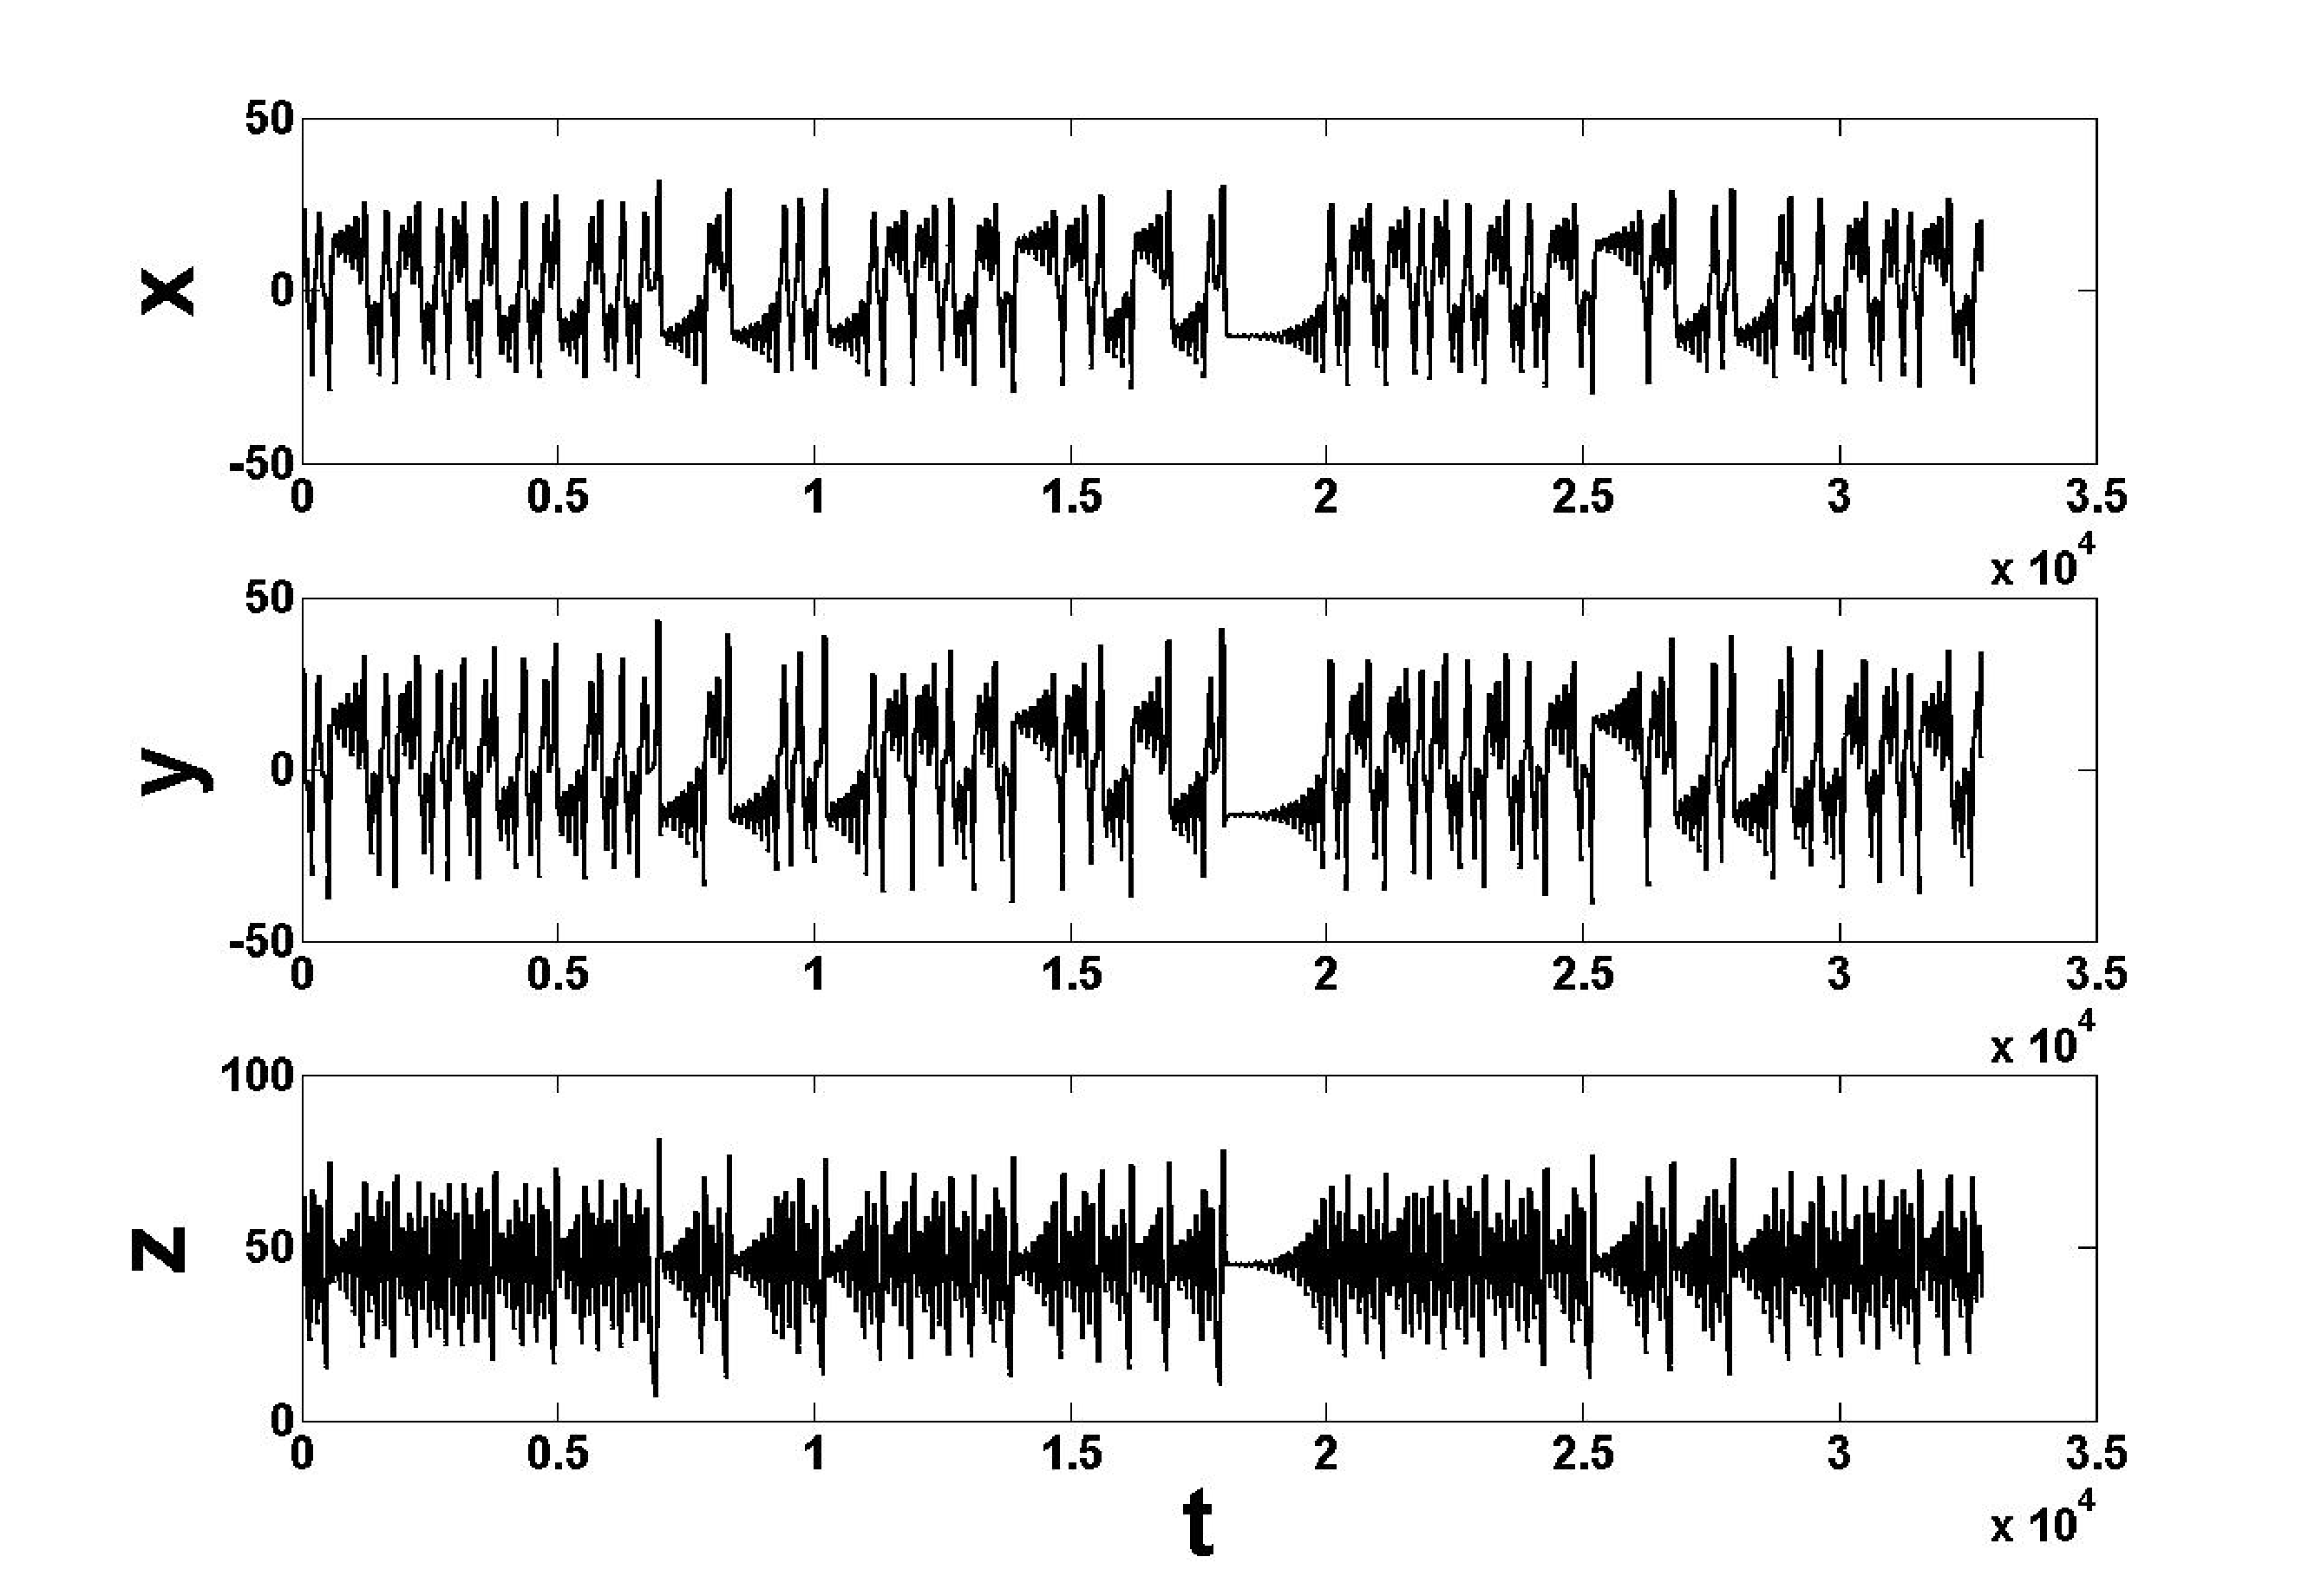
\includegraphics[width=1\columnwidth]{LorenzTiempo.pdf}\\
    \caption{Lorenz time series.}\label{fig:tiempo}
\end{figure}

\begin{figure}
    \centering
    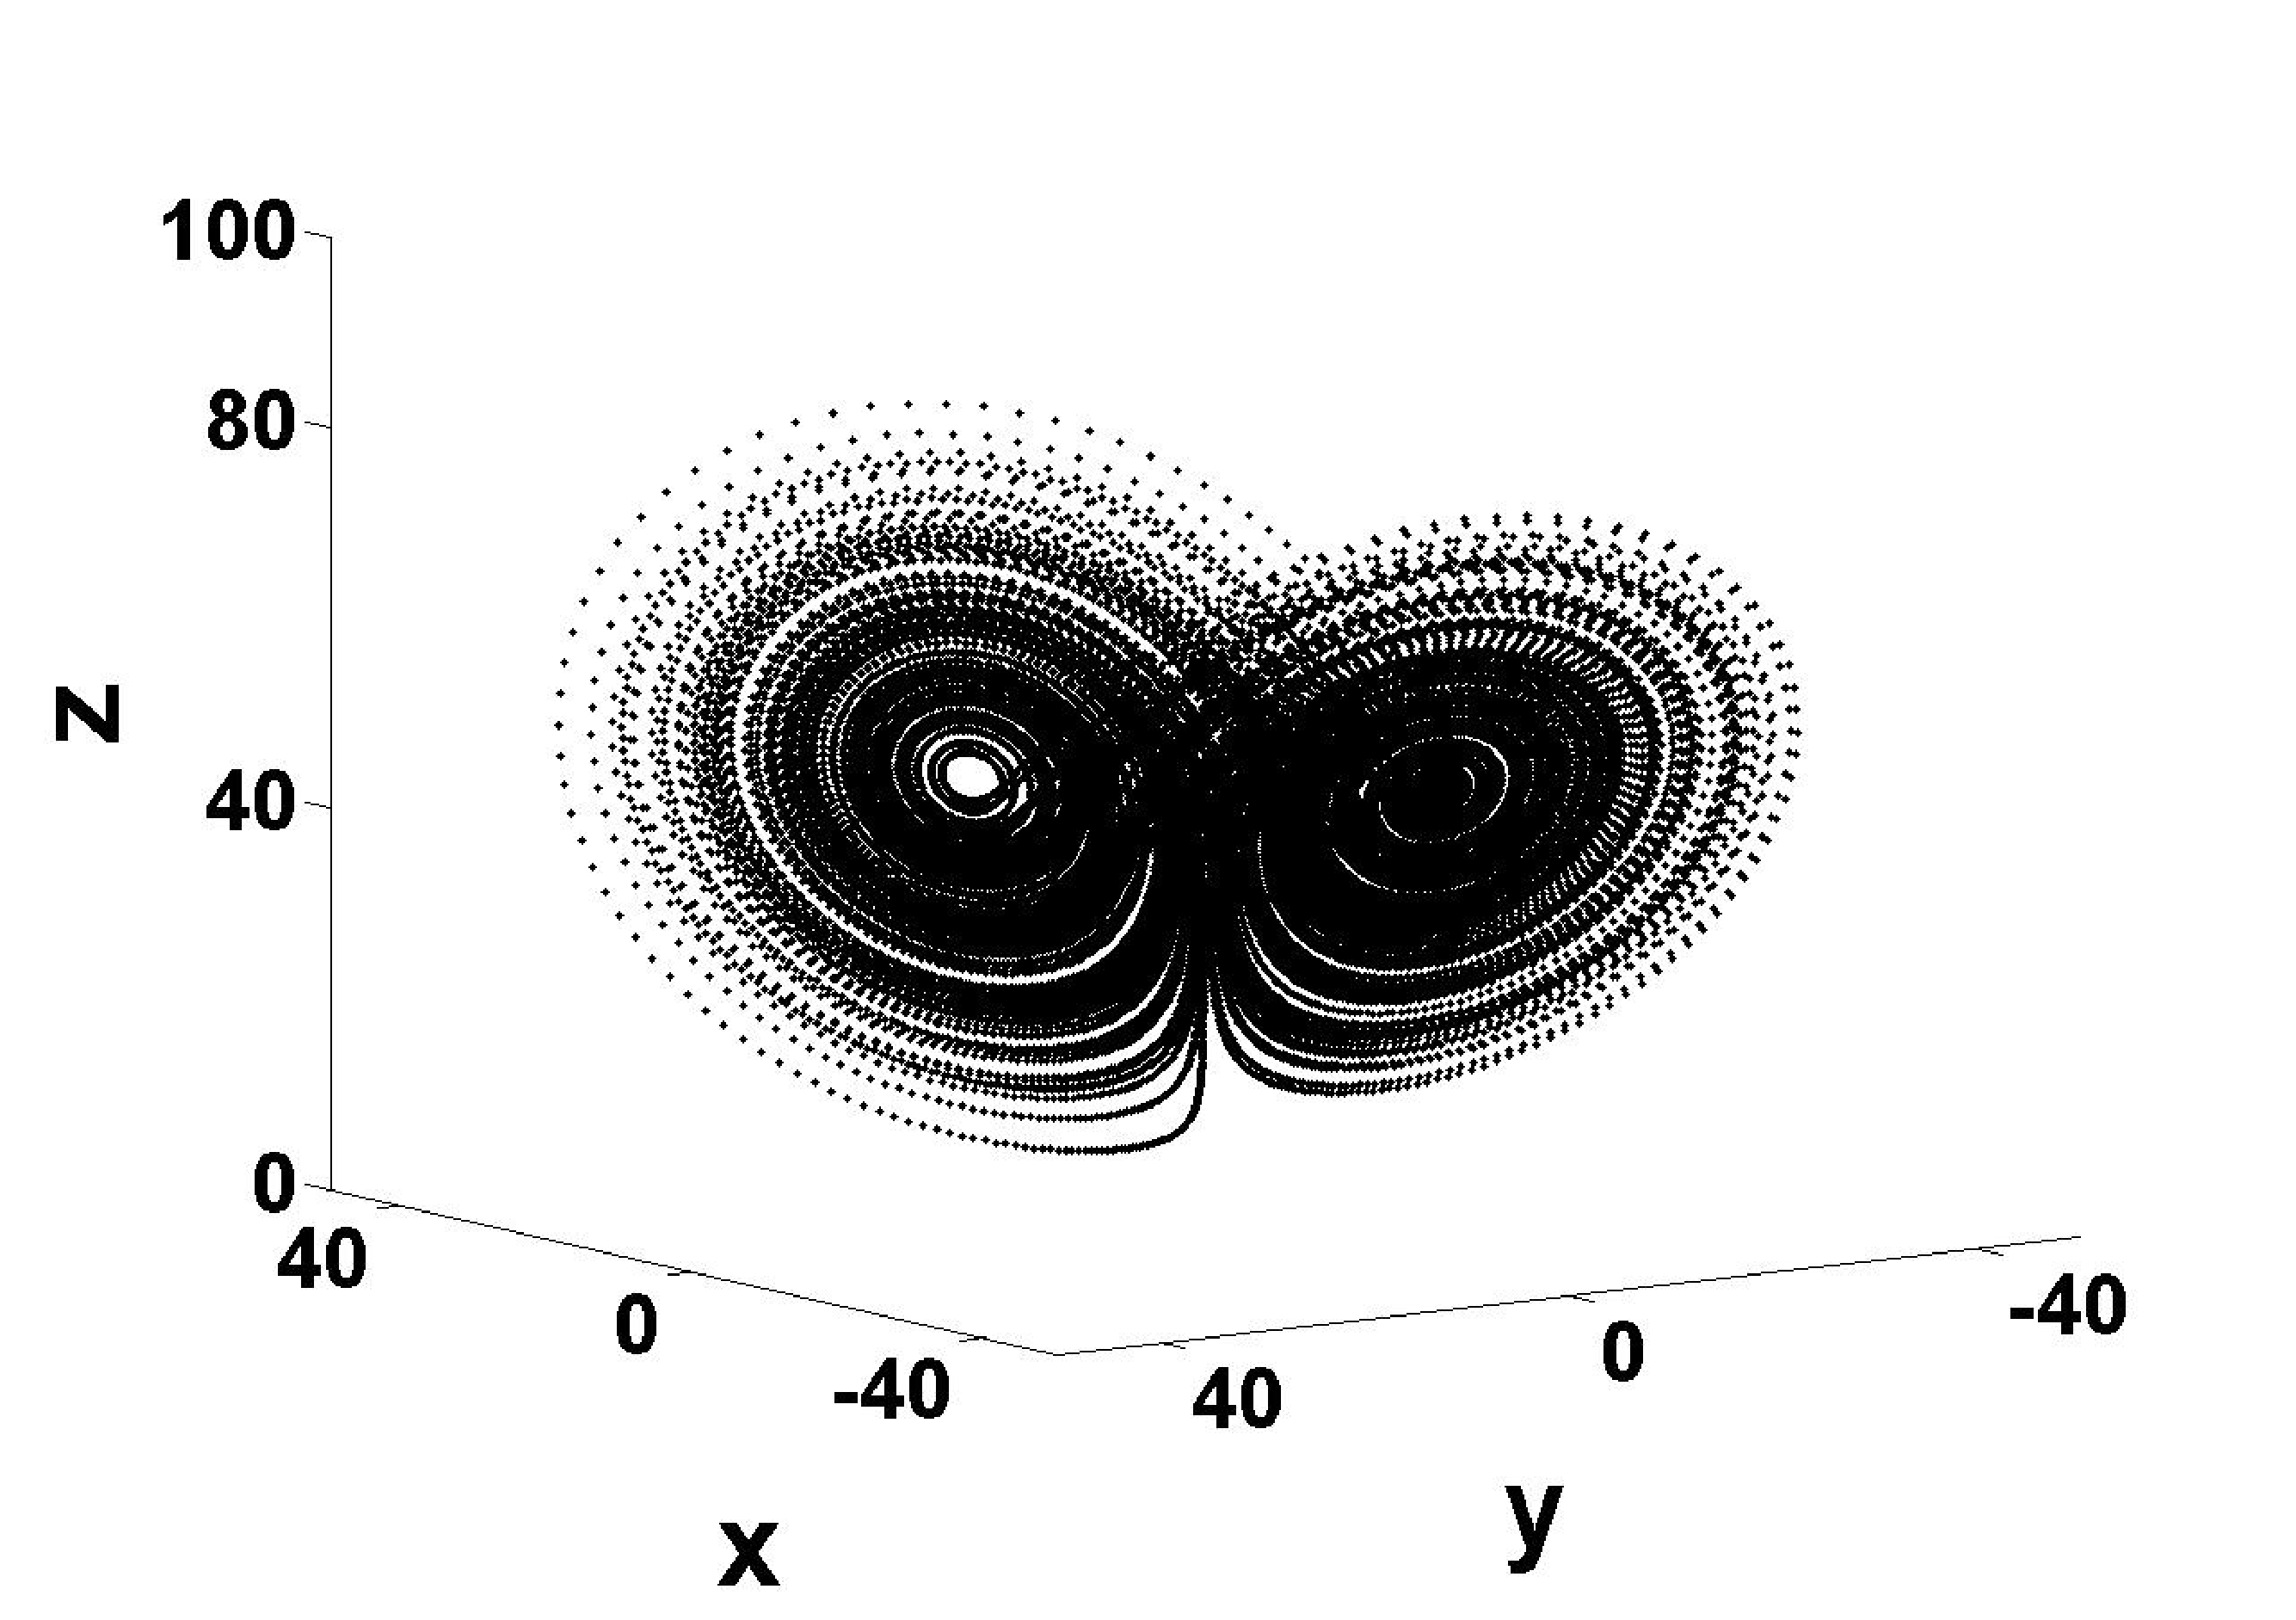
\includegraphics[width=1\columnwidth]{LorenzAtractor}\\
    \caption{Lorenz attractor.}\label{fig:atractor}
\end{figure}

\subsection{Conclusions}
\label{sec:conclusions} From the results presented herein, it is
possible to conclude that to obtain a PRNG optimum results
correspond to the integer arithmetics representation in both
hardware (resources and frequency) and statistical properties. The
\textit{concatenating} randomization technique makes the quality
independent of $\Delta t$ for this numeric representation.  For
\textit{discarding} randomization technique good results are
obtained  only for big values of $\Delta t$. The same happens for
fixed point implementations with both randomization techniques.

In terms of usage resources and frequency limitations integer
arithmetics performance is considerable better than floating point
and fixed point. Let us remark that to minimize resources
preprocessing of the chaotic system is required (scaling and
polarization) to get dividers that are a power of $2$, as
explained in subsection  \ref{sec:impleInt}.

On the other hand, for the floating point arithmetic's case  the
exponent is discarded in all the used randomization techniques and
consequently the dynamics is highly perturbed by the randomization
process. Then, as shown in Table \ref{tabla:Tabla2} $\Delta t$ is
not the relevant variable to predict a good or a bad PRNG.